\documentclass[ThesisDJ.tex]{subfiles}

\begin{document}
    Dieser Abschnitt dokumentiert die Durchführung des Projektes und zeigt dabei getroffene Maßnahmen zur Überwachung und Steuerung des Projektfortschrittes auf.\\
    Ziel ist es dabei, sicherzustellen, dass Abweichungen von der erfolgten Projektplanung und den damit in Verbindung stehenden Zielen so früh wie möglich erkannt 
    werden und ein Gegensteuern möglich ist \cite[S.~55ff]{riedl_management_2019}. In Kombination mit einer strukturierten Projektdurchführung, die die Umsetzung von 
    getroffenen Maßnahmen gewährleistet, soll der Projekterfolg messbar und kontrollierbar werden.

    \subsection{Theoretische Grundlagen des Projektcontrollings}
    Projektcontrolling beschreibt Maßnahmen, Regeln und Abläufe, die sicherstellen sollen, dass Projektziele
    erreicht werden \cite{kerzner_project_2022} \cite[S.~189]{kuster_handbuch_2022}. Dabei unterscheidet sich die konkrete Ausprägung 
    je nach verwendetem Vorgehensmodell. Bei einer traditionellen Vorgehensweise ist Projektcontrolling ein eigenständiger Prozess im Ablauf, welcher
    als Zyklus mit drei Etappen visualisiert werden kann, wie bspw. in Abbildung \ref{fig:controlling} zu sehen ist \cite[S.~191]{kuster_handbuch_2022}.

    \begin{figure}
        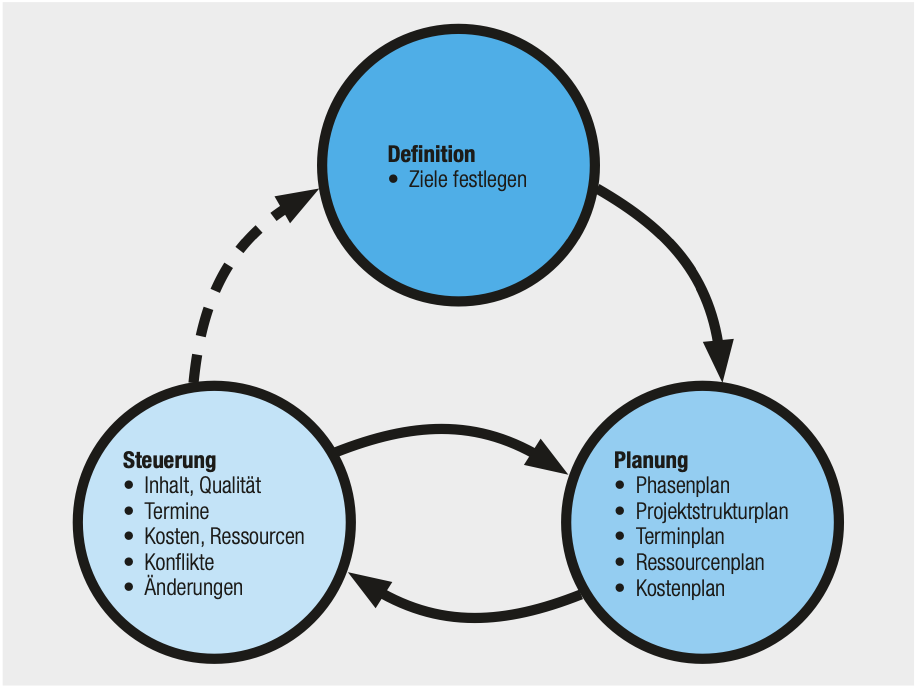
\includegraphics[scale=0.8]{controlling.png}
        \centering
        \caption{Die drei Etappen des Projektcontrollings}
        \label{fig:controlling}
    \end{figure}

    Der Controllingzyklus beginnt mit der Definitionsphase, in der eine korrekte und möglichst vollständige Vereinbarung zwischen dem Projektteam und dem 
    Auftraggeber ausgearbeitet wird. Diese Vereinbarung stellt dann die Basis für die konkrete Projektplanung, bei der im traditionellen Vorgehensmodell
    verbindliche Dokumente erstellt werden, welche für die Steuerung des Projektes als Maßstab herangezogen werden. Die eigentliche Steuerung 
    vergleicht dann kontinuierlich den Soll-Zustand mit dem aktuellen Ist-Zustand. Bei Abweichungen wird ein neuer Durchlauf des Zykluses angestoßen, bei dem die 
    Abweichungen in der Planungphase addressiert werden. Dadurch entstehen neue Planungsdokumente, welche dann für das weitere Steuern herangezogen werden. Dieser Zyklus wiederholt sich 
    bis zum Ende des Projektes \cite[S.~217]{dechange_projektmanagement_2024}. \\

    Im Gegensatz zum klassischen Projektcontrolling, das als ein klar abgegrenzter und zyklischer Prozess mit definierten Phasen (Definition, Planung, Steuerung) verstanden wird, 
    zeichnet sich das agile Controlling durch eine flexible und iterative Vorgehensweise aus. 
    Während im traditionellen Modell die Steuerung in regelmäßigen, aber längeren Intervallen (z.B. in Form von Soll-Ist-Vergleichen) erfolgt,
    sind im agilen Umfeld die Controllingmaßnahmen in den gesamten Arbeitsprozess integriert und erfolgen in kürzeren, oft iterativen Zyklen.
    Typische Werkzeuge für agiles Controlling sind Element wie Daily Standups, Reviews und Retrospektiven. Diese Werkzeuge kommen als feste Bestandteile 
    des agilen Arbeitsablaufes vor. Ein eigenständiger Zyklus wie bei traditionellen Vorgehensmodellen, wird hier nicht angewendet.

    \subsection{Methoden zur Erfassung des Projektfortschritts}
    Es gibt verschiedene Methodiken, mit denen im Rahmen des Projektcontrollings eine Fortschrittsbewertung durchgeführt werden kann.
    In diesem Abschnitt werden exemplarisch einige Methodiken vorgestellt, um im Anschluss aufzuzeigen, wie mit Ihnen eine Steuerung des Projektes durchgeführt 
    wurde.

    \subsubsection{Earned-Value-Analyse}
    Die Earned-Value-Analyse ist eine Methode zur Fortschrittsbewertung von Projekten, welche auf dem sogenannten \emph{magischen Dreieck} basiert. Dieses 
    besteht aus den drei Ecken \emph{Scope}, \emph{Kosten} und \emph{Zeit}, wie in Abbildung \ref{fig:magic_tri} zu sehen ist \cite[S.~84]{kuster_handbuch_2022}.
    In einer Earned-Value-Analyse wird dabei der \emph{erreichte Mehrwert} berechnet, d.h. wie viel konnte 
    in einer Zeitperiode vom Projekt fertiggestellt. Dies wird in Verhältnis zu dem im Voraus geplanten Aufwand und den verursachten Kosten 
    gesetzt. Wichtig dabei ist, dass nur vollständig abgeschlossene Arbeitspakete bzw. Meilensteine berücksichtigt werden.
    
    \begin{figure}
        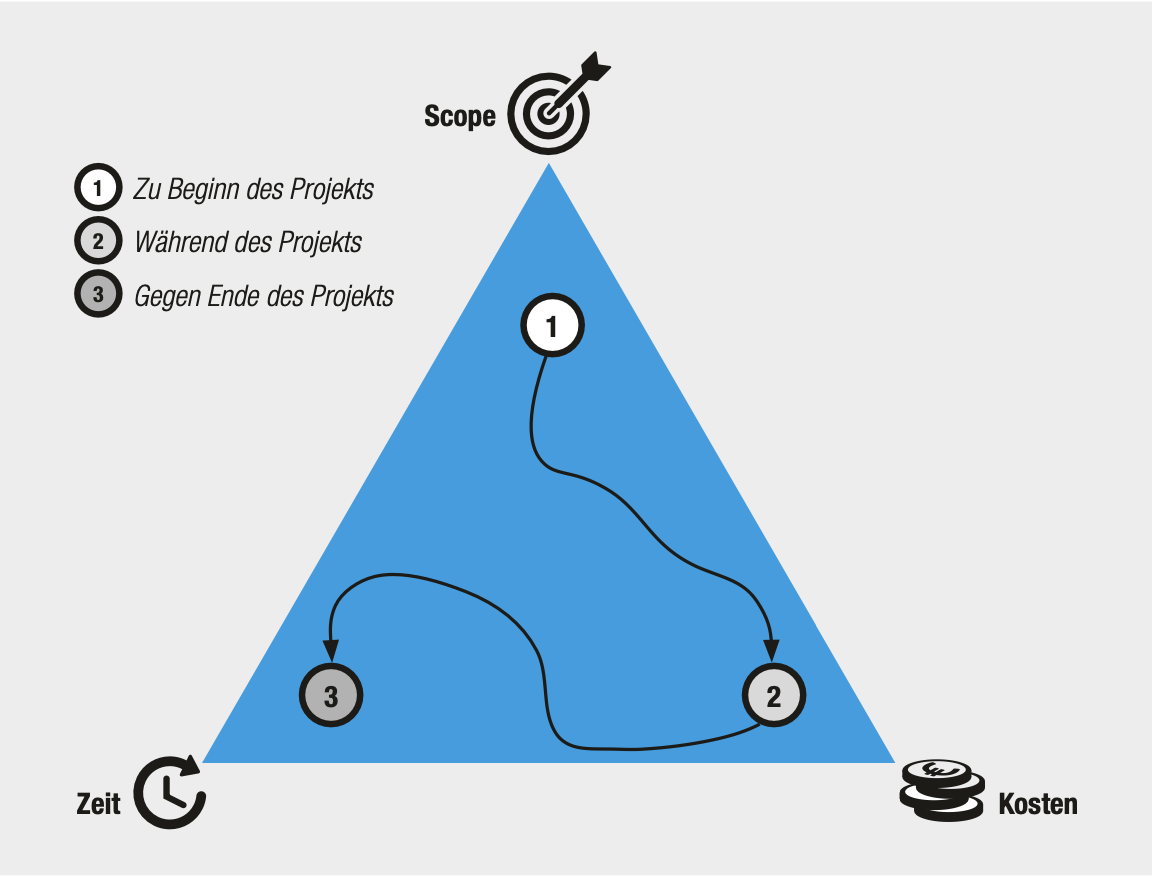
\includegraphics[scale=0.5]{magic_tri.png}
        \centering
        \caption{Das magische Dreieck}
        \label{fig:magic_tri}
    \end{figure}

    \subsubsection{Meilensteintrendanalyse}


\end{document}
